\documentclass[pdflatex,sn-nature]{sn-jnl}

%%%% Standard Packages
\usepackage{graphicx}%
\usepackage{multirow}%
\usepackage{amsmath,amssymb,amsfonts}%
\usepackage{booktabs}%
\usepackage{longtable}%
\usepackage{array}%
\usepackage{xcolor}%
\usepackage{textcomp}%

\raggedbottom

% ----------------------------
% Project metadata
% ----------------------------
\newcommand{\papertitle}{[Main paper title]}
\newcommand{\shortsititle}{Supplementary Information}

\title[Supplementary Information]{\shortsititle\\ for\\ \papertitle}

\author*[1]{\fnm{Author} \sur{One}}\email{email@example.com}
\author[2]{\fnm{Author} \sur{Two}}
\author[1,2]{\fnm{Author} \sur{Three}}
\author[1]{\fnm{Corresponding} \sur{Author}}\email{email@example.com}

\affil*[1]{\orgdiv{Department}, \orgname{Affiliation 1}, \orgaddress{\city{City}, \country{Country}}}
\affil[2]{\orgdiv{Department}, \orgname{Affiliation 2}, \orgaddress{\city{City}, \country{Country}}}

\abstract{This supplementary file provides additional methods, model inputs, assumptions, and policy-friction details supporting the main manuscript.}

\begin{document}

\maketitle

% ============================================================
% AGENT NOTES (delete before submission if desired)
% ============================================================
% Use this file only for supporting content that strengthens, validates,
% or documents claims made in the main paper.
%
% Good SI content includes:
% - supplementary methods details
% - robustness checks
% - alternative specifications
% - extended pair-level / city-level results
% - variable definitions / codebooks
% - extra figures / tables
% - implementation details not essential in the main text
%
% Avoid:
% - introducing a brand-new central claim that is not anchored to the main paper
% - contradicting the main manuscript
% - moving critical main-paper results here without reason
%
% Writing rules:
% - Keep structure parallel to the main paper when useful
% - Use clear sectioning and explicit labels (Fig. S1, Table S1, etc.)
% - Be traceable to repository files and scripts
% - Use [CHECK] rather than guessing
% ============================================================

\section*{The Supplementary file includes:}
% Briefly explain what this SI contains and how it complements the main paper.
[Supplementary overview placeholder]

\tableofcontents

\clearpage

\section*{List of sections:}
% Briefly explain what this SI contains and how it complements the main paper.
[Supplementary overview placeholder]

\tableofcontents

\clearpage

\section{Details of computer-vision-driven rooftop PV identification}
% Add details that support but are not essential for the main-text Methods.

\subsection{Coverage and segmentation support}

\begin{figure}[h!]
\centering
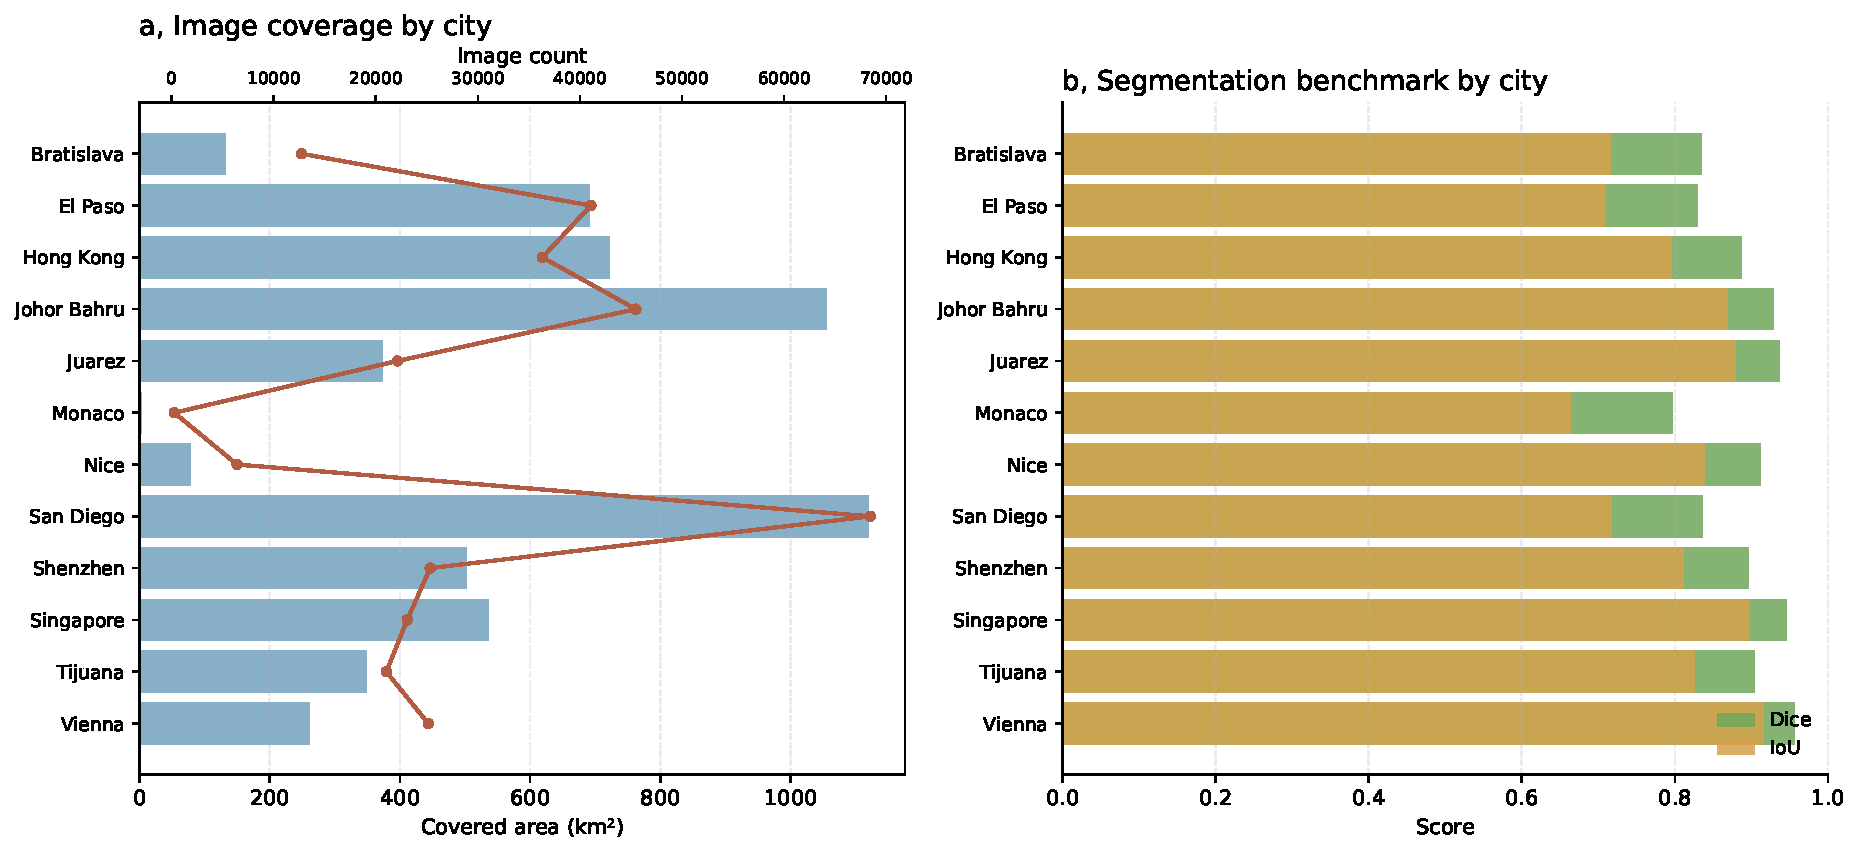
\includegraphics[width=\textwidth]{../figures/supplement/fig_s1_pv_identification_support.pdf}
\caption{\textbf{Supplementary support for computer-vision-driven rooftop PV identification.} \textbf{a, City-level image coverage varies across the 12 manuscript cities.} Bars report image count and the line reports covered area in square kilometres. \textbf{b, City-level segmentation benchmark performance supports the use of the PV mapping model across the study cities.} Horizontal bars report Dice and intersection-over-union (IoU) scores by city.}
\label{fig:s1_pv_identification_support}
\end{figure}

The manuscript analysis used 327,413 orthophoto image tiles across the 12 border cities, covering 5,822.3 km$^2$ of mapped urban area (Supplementary Fig.~\ref{fig:s1_pv_identification_support}a). City-level benchmark results were evaluated on held-out labelled image tiles and are summarized in Supplementary Fig.~\ref{fig:s1_pv_identification_support}b. The manuscript-city annotation set contains 623 labelled tiles across the 12 study cities (Table~\ref{tab:s4_annotation_dataset_stats}). These coverage, annotation and benchmark summaries support the main-text use of a computer-vision-driven PV layer as the spatial basis for pairwise rooftop PV comparisons.

\begin{table}[h!]
\centering
\caption{\textbf{Annotated rooftop PV segmentation dataset.} Labelled tiles are read from \texttt{data/annotations}; PV-positive tiles contain at least one pixel with grayscale value greater than 127. PV-pixel share is calculated over all annotated pixels in each city.}
{\small
\begin{tabular}{lrrrr}
\toprule
City & Labelled tiles & PV-positive tiles & PV pixels & PV-pixel share (\%) \\
\midrule
Bratislava & 78 & 31 & 87,638 & 0.429 \\
El Paso & 41 & 23 & 22,073 & 0.205 \\
Hong Kong & 34 & 14 & 73,194 & 0.821 \\
Johor Bahru & 37 & 17 & 67,402 & 0.695 \\
Juarez & 47 & 23 & 34,706 & 0.282 \\
Monaco & 54 & 15 & 73,541 & 0.520 \\
Nice & 47 & 18 & 33,246 & 0.270 \\
San Diego & 42 & 33 & 91,725 & 0.833 \\
Shenzhen & 59 & 15 & 218,559 & 1.413 \\
Singapore & 50 & 18 & 253,174 & 1.932 \\
Tijuana & 55 & 17 & 52,393 & 0.363 \\
Vienna & 79 & 35 & 375,979 & 1.815 \\
\midrule
Total & 623 & 259 & 1,383,630 & 0.847 \\
\bottomrule
\end{tabular}
}

\label{tab:s4_annotation_dataset_stats}
\end{table}

\subsection{Segmentation model training and inference}

Rooftop PV segmentation was implemented as a binary semantic-segmentation task. Training image--mask pairs were read from the annotation CSV and corresponding image and annotation roots. Label masks were converted to binary arrays by treating pixels with grayscale values above 127 as PV. The model was loaded through the local SegFormer model wrapper with a multi-dataset pretrained segmentation checkpoint, normalized using the model-specific mean and standard deviation, and fine-tuned without resizing the input tiles. The principal model, training, inference, vectorization and building-assignment parameters are summarized in Table~\ref{tab:s5_segmentation_model_parameters}.

\begin{table}[h!]
\centering
\caption{\textbf{Rooftop PV segmentation and building-assignment parameters.} Settings are taken from \texttt{train\_border\_supervised.py}, \texttt{inference.py}, \texttt{convert\_mask\_json.py} and \texttt{postprocess\_results\_on\_buildings.py}.}
{\small
\begin{tabular}{p{0.30\linewidth}p{0.62\linewidth}}
\toprule
Component & Setting \\
\midrule
Model & SegFormer semantic-segmentation model loaded through the local model wrapper with multi-dataset pretrained weights \\
Task & Binary rooftop PV segmentation \\
Input tiles & Orthophoto image tiles; no resizing during fine-tuning or inference normalization \\
Label construction & Grayscale annotation pixels $>127$ treated as PV; remaining pixels treated as background \\
Train/validation/test split & 0.8/0.1/0.1 random split; seed 42 \\
Loss & $(1-w_{\mathrm{Dice}})$ binary cross-entropy with logits + $w_{\mathrm{Dice}}$ Dice loss; $w_{\mathrm{Dice}}=0.5$ \\
Class weighting & Positive-pixel weight $=4.0$ in binary cross-entropy \\
Optimizer and schedule & AdamW; weight decay $=0.01$; cosine learning-rate schedule with 5\% warm-up \\
Training batch structure & Batch size $=2$; gradient accumulation $=16$; 40 epochs \\
Encoder schedule & Encoder frozen for the first 10 epochs, then unfrozen \\
Learning rates & Decode head $=6\times10^{-5}$; encoder $=4\times10^{-5}$ after unfreezing \\
Checkpoint selection & Best checkpoint selected by validation Dice; final checkpoint also retained \\
Inference threshold & Sigmoid probability threshold $=0.5$ \\
Inference batch structure & Batch size $=8$; 16 workers where available \\
Mask vectorization & Raster-to-polygon conversion from Mercator tile bounds to WGS84 polygons; invalid geometries repaired and overlapping polygons dissolved \\
Building assignment & Segments $<2.5$~m$^{2}$ removed; nearest-building assignment in EPSG:3857 within 5~m \\
\bottomrule
\end{tabular}
}

\label{tab:s5_segmentation_model_parameters}
\end{table}

For city-scale inference, the trained SegFormer model was applied to all available orthophoto tiles for each target city. The model output logits were interpolated to the input image size where needed, converted to probabilities using a sigmoid transform, and thresholded at 0.5 to produce binary PV masks. The resulting binary mask tiles were written under the corresponding city output directory and used as inputs to the vectorization step.

\subsection{Mask vectorization and building-level assignment}

Predicted binary mask tiles were converted to georeferenced PV polygons using the Mercator tile coordinates. For each tile, the tile bounds were converted to WGS84 coordinates, an affine transform was constructed from the tile bounds and mask dimensions, and connected PV regions were vectorized with raster-to-polygon conversion. Invalid geometries were repaired, and non-empty tile-level feature collections were merged into a city-level GeoJSON layer. Adjacent or overlapping PV geometries were dissolved with a unary union before writing the city-level \texttt{results.geojson} output.

City-level PV polygons were then linked to building footprints. During building assignment, PV segments smaller than 2.5 m$^2$ were removed, distances were calculated in EPSG:3857, and each remaining PV segment was assigned to the nearest building if the distance was no greater than 5 m. The output retained all segments and stored the matched building index and nearest-building distance, allowing unmatched PV polygons to remain available for quality checks. Across the 12 manuscript cities, 242,921 PV segments were matched to buildings and 33,740 remained unmatched after this nearest-building assignment step.

\subsection{Building-use harmonization and PV metrics}

Building-use classes were harmonized from Open Building Map occupancy codes into six base classes. Occupancy codes beginning with RES were mapped to residential classes, with RES2 and RES3 assigned to multi-residential and other RES codes assigned to single-residential. Codes beginning with COM, IND, GOV and EDU were mapped to commercial, industrial, and public or infrastructure classes, respectively. AGR, ASS, MIX and UNK codes were assigned to the others class. Main-text residential analyses grouped single-residential and multi-residential buildings, while non-residential analyses grouped commercial, industrial, public or infrastructure, and others.

The core rooftop PV utilization metric was calculated as PV area divided by building area. City-level all-building utilization used total mapped PV area over total building area; residential and non-residential utilization used the corresponding PV-area and building-area totals by use group. Building-type PV adoption was calculated as the fraction of buildings in a base class with at least one mapped PV segment. Roof-size analyses used the same building-level PV linkage after assigning buildings to footprint-area bins. These definitions produce the city, pair, building-type and roof-size summaries used in the main-text Results.

\section{Details of urban PV economic modeling}

\subsection{Discounted cash-flow specification}

City-level PV economic outputs were generated from the same discounted cash-flow model used for the main-text Figure 4 comparisons. The model applies a standardized 5~kW rooftop PV system, 25-year project lifetime and 5\% discount rate to all 12 study cities, while allowing city-specific variation in installed cost, CAPEX reduction, electricity rate, export rate, PV yield, self-consumption ratio, degradation rate and O\&M rate. The model output is saved in \texttt{data/PV\_Eco\_model/economic\_analysis\_results.csv}; annual cash-flow trajectories are saved in \texttt{data/PV\_Eco\_model/discounted\_cashflow\_profiles\_city\_year.csv}.

For each city, gross CAPEX is calculated from system size and cost per watt, and net CAPEX subtracts the city-specific CAPEX-reduction share. Annual PV production declines by the city-specific degradation rate. Annual value is computed from a blended solar value that weights the retail electricity rate by the self-consumed share and the export rate by the exported share. O\&M is represented as a fixed annual share of gross CAPEX. The resulting annual net cash-flow sequence is used to calculate LCOE, NPV, IRR, simple payback and discounted payback. These outputs provide the economic-return variables used in the rank comparison, gap analysis, Figure 4 economic contrasts and Supplementary Table S3 counterfactuals.

\subsection{City-level model inputs}

\begin{table}[h!]
\centering
\caption{\textbf{City-level economic model inputs used in the rooftop PV analysis.} Cost/W is installed cost in US\$~W$^{-1}$, CAPEX red. is the capital-cost reduction share, electricity and export rates are in US\$~kWh$^{-1}$, yield is kWh~kW$^{-1}$~yr$^{-1}$, self-cons. is the self-consumption share, degrad. is the annual degradation rate, and O\&M is the annual operations-and-maintenance cost as a share of gross CAPEX.}
{\scriptsize
\begin{longtable}{lrrrrrrrr}
\toprule
City & Cost/W & CAPEX red. & Elec. rate & Export rate & Yield & Self-cons. & Degrad. & O\&M \\
\midrule
\endfirsthead
\toprule
City & Cost/W & CAPEX red. & Elec. rate & Export rate & Yield & Self-cons. & Degrad. & O\&M \\
\midrule
\endhead
Bratislava & 1.90 & 0.10 & 0.194 & 0.173 & 1150 & 0.70 & 0.005 & 0.010 \\
El Paso & 2.34 & 0.20 & 0.130 & 0.020 & 1750 & 0.70 & 0.005 & 0.010 \\
Hong Kong & 2.50 & 0.20 & 0.183 & 0.350 & 1350 & 0.70 & 0.005 & 0.010 \\
Johor Bahru & 1.00 & 0.15 & 0.057 & 0.070 & 1450 & 0.70 & 0.005 & 0.010 \\
Juarez & 1.60 & 0.10 & 0.119 & 0.119 & 1750 & 0.70 & 0.005 & 0.010 \\
Monaco & 2.60 & 0.20 & 0.280 & 0.173 & 1500 & 0.70 & 0.005 & 0.010 \\
Nice & 2.20 & 0.20 & 0.278 & 0.173 & 1500 & 0.70 & 0.005 & 0.010 \\
San Diego & 2.60 & 0.20 & 0.390 & 0.030 & 1650 & 0.70 & 0.005 & 0.010 \\
Shenzhen & 0.60 & 0.15 & 0.077 & 0.070 & 1350 & 0.70 & 0.005 & 0.010 \\
Singapore & 1.20 & 0.10 & 0.241 & 0.219 & 1450 & 0.70 & 0.005 & 0.010 \\
Tijuana & 1.60 & 0.10 & 0.119 & 0.119 & 1650 & 0.70 & 0.005 & 0.010 \\
Vienna & 2.20 & 0.20 & 0.292 & 0.216 & 1150 & 0.70 & 0.005 & 0.010 \\
\bottomrule
\end{longtable}
}

\label{tab:s1_economic_model_city_inputs}
\end{table}

\subsection{Global model assumptions}

\begin{table}[h!]
\centering
\caption{\textbf{Global assumptions used in the discounted cash-flow analysis.} These assumptions are held constant across cities so that within-pair differences reflect city-level cost, tariff, incentive and PV-yield inputs rather than different project scales or lifetimes.}
{\small
\begin{tabular}{llll}
\toprule
Assumption & Value & Unit & Provenance \\
\midrule
system\_size\_kw & 5.0 & kW & plot\_discounted\_cashflow\_profiles\_citypair\_lines.py default \\
project\_lifetime\_years & 25.0 & years & plot\_discounted\_cashflow\_profiles\_citypair\_lines.py default \\
discount\_rate & 0.05 & share & plot\_discounted\_cashflow\_profiles\_citypair\_lines.py default \\
\bottomrule
\end{tabular}
}

\label{tab:s1_global_model_assumptions}
\end{table}

\subsection{IRR catch-up requirement decomposition by border-city pair}

\begin{table}[h!]
\centering
\caption{Pair-level requirements for the lagging city to match the leading city's IRR under two one-factor counterfactuals: export-rate adjustment and PV CAPEX subsidy. The table reports both absolute extra export rate and relative extra export requirement (\%). For readability, the pair key column is omitted in the rendered table. Results are generated from \texttt{plot\_irr\_match\_requirement\_heatmap.py} using the same base economic assumptions as the main analysis (system size $=5$ kW, project lifetime $=25$ years, discount rate $=0.05$).}
{\scriptsize
\begin{longtable}{lrrrrrrrrrr}
\toprule
Lagging $\leftarrow$ Leading & Lead IRR (\%) & Lag IRR (\%) & Gap (pp) & Curr. export (\$/kWh) & Req. export (\$/kWh) & Extra export (\$/kWh) & Extra export / curr. (\%) & Req. subsidy (\$) & Subsidy / gross & Total CAPEX red. \\
\midrule
\endfirsthead
\toprule
Lagging $\leftarrow$ Leading & Lead IRR (\%) & Lag IRR (\%) & Gap (pp) & Curr. export (\$/kWh) & Req. export (\$/kWh) & Extra export (\$/kWh) & Extra export / curr. (\%) & Req. subsidy (\$) & Subsidy / gross & Total CAPEX red. \\
\midrule
\endhead
Tijuana $\leftarrow$ San Diego & 20.41 & 11.21 & 9.20 & 0.119 & 0.369 & 0.250 & 210.1 & 2,933 & 0.367 & 0.467 \\
El Paso $\leftarrow$ Juarez & 12.14 & 5.44 & 6.70 & 0.020 & 0.217 & 0.197 & 986.4 & 3,890 & 0.332 & 0.532 \\
Hong Kong $\leftarrow$ Shenzhen & 17.85 & 13.39 & 4.46 & 0.350 & 0.556 & 0.206 & 58.9 & 2,239 & 0.179 & 0.379 \\
Johor Bahru $\leftarrow$ Singapore & 29.80 & 7.26 & 22.54 & 0.070 & 0.483 & 0.413 & 590.0 & 2,962 & 0.592 & 0.742 \\
Monaco $\leftarrow$ Nice & 19.00 & 15.71 & 3.29 & 0.173 & 0.317 & 0.144 & 83.5 & 1,649 & 0.127 & 0.327 \\
Bratislava $\leftarrow$ Vienna & 15.40 & 10.05 & 5.35 & 0.173 & 0.412 & 0.239 & 138.2 & 2,527 & 0.266 & 0.366 \\
\bottomrule
\end{longtable}
}

\label{tab:s3_irr_match_requirements_by_pair}
\end{table}

\subsection{Supplementary CAPEX--NPV uncertainty comparison}

\begin{figure}[h!]
\centering
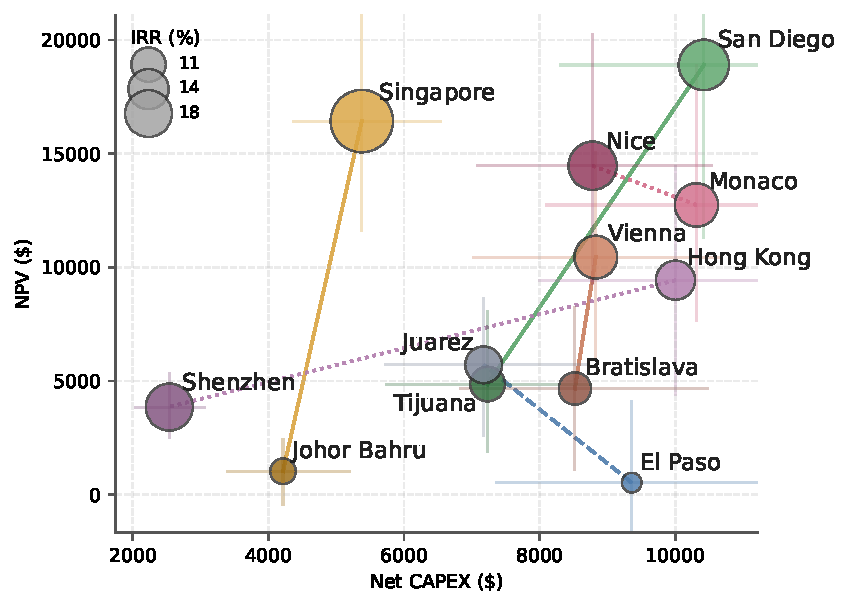
\includegraphics[width=0.9\textwidth]{../figures/supplement/capex_vs_profitability_with_errorbar.pdf}
\caption{Uncertainty-propagated analogue of main-text Figure 4a. Median net CAPEX and NPV are shown for each city with horizontal and vertical 95\% uncertainty intervals; marker area scales with median IRR, and paired cities remain linked as in the main-text comparison. Intervals are derived from 1,000 Monte Carlo draws per city using the same economic model as the main text while perturbing key inputs around their base values: cost per watt (10\% relative standard deviation), PV yield (5\%), electricity rate (10\%), export rate (15\%), self-consumption ratio ($\pm$0.05), CAPEX reduction ($\pm$0.03), and O\&M rate ($\pm$0.002), with draws clipped to plausible bounds. The relative separation between the strongest and weakest city cases remains visible under these perturbations.}
\label{fig:s2_economic_uncertainty_capex_npv}
\end{figure}

\section{Details of policy friction analysis}

\subsection{City-side friction matrix construction}

The policy-friction matrix contains one row for each city side of the six border-city pairs. Scores were assigned from official policy documents, utility guidance, permitting pages and program materials, with the source notes and URLs retained in \texttt{data/Policy\_frictions/border\_city\_pv\_friction\_matrix.csv}. Each component uses the common 0--3 rubric shown in Supplementary Table~S2, where higher values indicate greater friction. Revenue-side components A--D capture export compensation, export constraints, settlement complexity and policy uncertainty. Administrative components E--H capture small-system approval, building or planning approval, grid study or fee requirements and professional credential requirements.

The Revenue Friction Index is the sum of components A--D, the Administrative Friction Index is the sum of components E--H and the Total Friction Index is their sum. The main-text heatmap reports the eight component scores and the three summary indices in this order: A--D, Revenue, E--H, Administrative and Total. Within-pair policy-friction rankings use the Total Friction Index with lower values treated as more favorable; tied values receive the same neutral rank. Pair-level gap figures use signed differences in the fixed pair order specified by the plotting scripts, so negative friction gaps indicate lower friction on the first-listed city side. These indices are used only as documented-rule summaries and should not be interpreted as direct measurements of realized approval duration, informal enforcement or adopter experience.

\subsection{Policy-friction codebook and scoring rubric}

{\scriptsize
\begin{longtable}{p{0.45cm}p{1.85cm}p{0.95cm}p{2.0cm}p{2.0cm}p{2.0cm}p{2.0cm}p{2.0cm}}
\toprule
Ind. & Short name & Dim. & Score 0 & Score 1 & Score 2 & Score 3 & Interpretation \\
\midrule
\endfirsthead
\toprule
Ind. & Short name & Dim. & Score 0 & Score 1 & Score 2 & Score 3 & Interpretation \\
\midrule
\endhead
A & Export compensation friction & Revenue & Stable and attractive compensation (e.g., generous FiT or close-to-retail offset). & Moderate discount relative to retail value. & Clearly weaker export value than self-consumption, but still usable. & Very weak export compensation or highly unfavorable export pricing. & Higher values indicate weaker monetization of exported generation. \\
B & Export constraint friction & Revenue & No meaningful constraint on offset, carry-forward, or monetization. & Minor or occasional constraints. & Noticeable limits on export use or contractual caps. & Strong limits such as no cash-out, no carry-forward, or strict export-capacity ceilings. & Captures whether exported electricity can be converted into durable economic value. \\
C & Settlement complexity friction & Revenue & Simple and predictable settlement (e.g., straightforward FiT or netting). & Mostly standardized settlement with limited complexity. & Multiple contractual or tariff steps materially affect settlement. & Highly complex settlement involving market exposure, layered contracts, or difficult bill reconciliation. & Captures whether monetization depends on complicated billing or market arrangements. \\
D & Policy uncertainty friction & Revenue & Stable long-term policy with clear continuation horizon. & Mostly stable framework with limited uncertainty. & Meaningful uncertainty due to reform risk or short policy horizons. & High uncertainty due to active reform, marketization, or unstable support mechanisms. & Captures how predictable future rooftop PV revenue streams are. \\
E & Small-system approval friction & Administrative & Clear simplified path or self-issue route for small systems. & Mostly simple approval process, with some documentation requirements. & Formal approval remains necessary and simplification is limited. & No meaningful simplification; small systems face full approval burden. & Designed to distinguish jurisdictions with streamlined residential permitting from those without. \\
F & Building/planning approval friction & Administrative & Minimal additional building/planning review in ordinary cases. & Some additional review only for specific conditions (e.g., heritage, structural change). & Routine administrative review or filing is typically required. & Multi-agency or substantial building/planning review is commonly required. & Captures urban-form and building-governance barriers beyond pure energy regulation. \\
G & Grid study/fee friction & Administrative & No material fee or study burden for typical rooftop systems. & Light utility processing or limited technical checks. & Meaningful fees, studies, or multiple utility steps for many systems. & Heavy study requirements, high fees, or substantial interconnection burden. & Reflects utility-facing transaction costs and soft costs. \\
H & Professional credential friction & Administrative & No unusual credential requirement beyond normal electrical practice. & Some certified participation is advisable or needed in limited cases. & Certified or licensed professionals are routinely required. & Multiple formal credentials, recognized intermediaries, or tightly restricted installer channels are required. & Captures labor-market and procedural gatekeeping. \\
\bottomrule
\end{longtable}
}


\end{document}
